% vim: set spell spelllang=en tw=100 et sw=4 sts=4 :

\def\year{2016}\relax
\documentclass[letterpaper]{article}
\usepackage{aaai16}
\usepackage{times}
\usepackage{helvet}
\usepackage{courier}

\usepackage{cleveref}
\usepackage{complexity}
\usepackage[ruled,vlined]{algorithm2e} % algorithms
\usepackage{booktabs}                  % less ugly tables
\usepackage[tight-spacing=true]{siunitx}
\usepackage{tikz}                      % For pretty pictures
\usepackage{gnuplot-lua-tikz}          % graphs

% \usepackage{showframe}

\usetikzlibrary{arrows, shadows, calc, positioning, decorations, decorations.pathmorphing,
decorations.pathreplacing, patterns, tikzmark, fit}

% \input isn't expandable. yay.
\makeatletter\newcommand*\inputhaxx[1]{\@@input #1}\makeatother

% labels in algorithms
\newcommand{\mclabel}[1]{\label{line:mc:#1}}
\newcommand{\mcline}[1]{line~\ref{line:mc:#1}}
\newcommand{\mclinerange}[2]{lines~\ref{line:mc:#1} to~\ref{line:mc:#2}}

% cref style
\crefname{algocf}{Algorithm}{Algorithm}
\Crefname{algocf}{Algorithm}{Algorithms}
\crefname{figure}{Figure}{Figures}
\Crefname{figure}{Figure}{Figures}
\crefname{table}{Table}{Tables}
\Crefname{table}{Table}{Tables}

% common names of things
\newcommand{\Cbest}{C^\star}
\newcommand{\bounds}{\mathit{bounds}}
\newcommand{\order}{\mathit{order}}
\newcommand{\colour}{\mathit{currentColour}}
\newcommand{\uncoloured}{\mathit{uncoloured}}
\newcommand{\colourable}{\mathit{colourable}}
\newcommand{\expand}{\FuncSty{expand}}
\newcommand{\dominated}{\FuncSty{dominated}}
\newcommand{\colourOrder}{\FuncSty{colour}}
\newcommand{\vrej}{v_{\mathit{rej}}}
\newcommand{\kwunset}{\KwSty{unset}}
\newcommand{\vertexset}{V}
\newcommand{\neighbourhood}{N}

% some pretty colours
\definecolor{safelightblue}{rgb}{0.65098, 0.807843, 0.890196}
\definecolor{safedarkblue}{rgb}{0.121569, 0.470588, 0.705882}
\definecolor{safelightgreen}{rgb}{0.698039, 0.87451, 0.541176}
\definecolor{safedarkgreen}{rgb}{0.2, 0.627451, 0.172549}
\definecolor{safelightorange}{rgb}{0.996078, 0.901961, 0.807843}
\definecolor{safedarkorange}{rgb}{0.54902, 0.176471, 0.015686}
\definecolor{safemediumorange}{rgb}{0.74902, 0.505882, 0.490196}
\definecolor{safeverydarkblue}{rgb}{0.007843, 0.219608, 0.345098}
\definecolor{safenearlywhite}{rgb}{0.9, 0.9, 0.9}
\definecolor{safelightgrey}{rgb}{0.7, 0.7, 0.7}

% drawing styles
\tikzset{vertex/.style={draw, circle, inner sep=0pt, minimum size=0.4cm, font=\small}}
\tikzset{notvertex/.style={vertex, color=white, text=black}}
\tikzset{plainvertex/.style={vertex}}
\tikzset{selectedvertex/.style={vertex, fill=safedarkblue}}
\tikzset{delvertex/.style={vertex, dotted, color=safelightgrey}}
\tikzset{vertexc1/.style={vertex, fill=safelightblue}}
\tikzset{vertexc2/.style={vertex, fill=safedarkblue, text=safenearlywhite}}
\tikzset{vertexc3/.style={vertex, fill=safelightorange}}
\tikzset{vertexc4/.style={vertex, fill=safedarkorange, text=safenearlywhite}}

\tikzset{edge/.style={color=safelightgrey}}
\tikzset{bedge/.style={very thick}}
\tikzset{deledge/.style={dotted, color=safelightgrey}}
\tikzset{edgel1/.style={color=safeverydarkblue}}
\tikzset{edgel2/.style={color=safemediumorange}}
\tikzset{edgel3/.style={very thick, color=safedarkblue}}
\tikzset{edgel4/.style={very thick, color=safelightorange}}

\tikzset{processarrow/.style={->, very thick, decorate, decoration={snake, post length=0.5mm}}}
\tikzset{brace/.style={decorate, decoration={brace}, very thick}}
\tikzset{label/.style={font=\small}}

\makeatletter\@ifpackageloaded{showframe}{
    % show lines down the middle columns too
    % http://tex.stackexchange.com/questions/16199/test-if-a-package-or-package-option-is-loaded
\newlength\Fcolumnseprule\setlength\Fcolumnseprule{0.4pt}\def\@outputdblcol{%
  \if@firstcolumn\global \@firstcolumnfalse \global \setbox\@leftcolumn \box\@outputbox
  \else
    \global \@firstcolumntrue
    \setbox\@outputbox \vbox{\hb@xt@\textwidth{\hb@xt@\columnwidth{\box\@leftcolumn \hss}%
    \vrule \@width\Fcolumnseprule\hfil{\normalcolor\vrule \@width\columnseprule}
    \hfil\vrule \@width\Fcolumnseprule\hb@xt@\columnwidth {\box\@outputbox \hss}}}\@combinedblfloats\@outputpage
    \begingroup\@dblfloatplacement\@startdblcolumn\@whilesw\if@fcolmade \fi{\@outputpage\@startdblcolumn}\endgroup
  \fi
}}{}
\makeatother

\renewcommand{\topfraction}{0.9}
\renewcommand{\bottomfraction}{0.8}
\renewcommand{\dbltopfraction}{0.9}
\renewcommand{\textfraction}{0.05}
\setcounter{dbltopnumber}{2}
\renewcommand{\floatpagefraction}{0.85}
\renewcommand{\dblfloatpagefraction}{0.85}

% \frenchspacing
\setlength{\pdfpagewidth}{8.5in}
\setlength{\pdfpageheight}{11in}
\pdfinfo{
/Title (Finding Maximum $k$-Cliques Faster Using Lazy Global Domination)
/Author (Ciaran McCreesh, Patrick Prosser)}
\setcounter{secnumdepth}{0}

\begin{document}
\title{Finding Maximum $k$-Cliques Faster Using Lazy Global Domination}
 \author{
    Ciaran McCreesh%
    \thanks{This work was supported by the Engineering and Physical Sciences Research Council [grant number EP/K503058/1]}
    \and
    Patrick Prosser
    \\ University of Glasgow, Glasgow, Scotland
}
\maketitle

\begin{abstract}
    A clique in a graph is a set of vertices, each of which is adjacent to every other vertex in
    this set. A $k$-clique relaxes this requirement, requiring vertices to be within a distance $k$
    of each other, rather than directly adjacent. In theory, a maximum clique algorithm can easily
    be adapted to solve the maximum $k$-clique problem, although large sparse $k$-clique graphs
    reduce to large dense clique graphs, which can be computationally challenging. We adapt a state of
    the art maximum clique algorithm to show that this reduction is in fact useful in practice, and
    introduce a lazy global domination rule which sometimes vastly reduces the search space. We
    include experimental results for a range of real-world and benchmark graphs, and a detailed look
    at random graphs. We also use thread-parallel search to solve some harder instances.
\end{abstract}

\section{Introduction}

A clique in a graph is a set of vertices, each of which is adjacent to every other vertex in the
set. Finding a clique of maximum size in a graph is one of the basic \NP-hard problems
\cite{Garey:1990}; applications include geometry, coding theory, computer vision and bioinformatics
\cite{Bomze:1999,Butenko:2006}. However, when analysing real-world data, a clique may be too strong
a requirement. A $k$-clique (or sometimes $n$-clique or $s$-clique---in an unfortunate clash of
notation, ``$k$-clique problem'' is sometimes used elsewhere for the decision version of the clique
problem, to distinguish it from the maximum clique problem) is a relaxed form of clique, where
instead of requiring each pair of vertices to be directly adjacent, we only require that they be
connected by a path of length at most $k$ \cite{Luce:1950}.  Thus a $1$-clique \emph{is} a clique, a
$2$-clique may be thought of as ``a group of people, all of whom either know each other or have a
mutual acquaintance'', and so on. We illustrate this in \cref{figure:k-cliques}.  Determining the
size of a maximum $k$-clique is \NP-hard for any fixed $k$ \cite{Bourjolly:2002}.

A related relaxation is a $k$-club, which tightens the requirement of a $k$-clique as follows
\cite{Mokken:1979}. In a $k$-clique, each pair of vertices is connected by a path of length at most
$k$, but that path may use any vertices in the original graph. In a $k$-club, each pair of vertices
must be connected by a path of length at most $k$ using only vertices that are also in the club.
Thus the $2$-clique in \cref{figure:k-cliques} is \emph{not} a $2$-club (obviously, every $k$-club
is a $k$-clique).

\begin{figure}[b!] % first page please
    \centering
    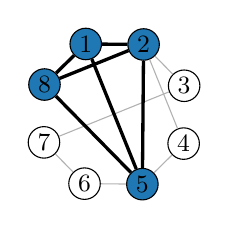
\begin{tikzpicture}[scale=0.8]
        \newcount \c
        \foreach \n in {1, ..., 8}{
            \c=\n \advance\c by -1 \multiply\c by -360 \divide\c by 8 \advance\c by 90 \advance\c by 22.5
            \ifthenelse{\n = 1 \OR \n = 2 \OR \n = 5 \OR \n = 8}{
                \node[selectedvertex] (N\n) at (\the\c:1.2) {\n};
            }{
                \node[plainvertex] (N\n) at (\the\c:1.2) {\n};
            }
        }

        \draw [edge] (N2) -- (N3);
        \draw [edge] (N2) -- (N4);
        \draw [edge] (N3) -- (N7);
        \draw [edge] (N4) -- (N5);
        \draw [edge] (N5) -- (N6);
        \draw [edge] (N6) -- (N7);

        \draw [bedge] (N1) -- (N2);
        \draw [bedge] (N1) -- (N5);
        \draw [bedge] (N1) -- (N8);
        \draw [bedge] (N2) -- (N5);
        \draw [bedge] (N2) -- (N8);
        \draw [bedge] (N5) -- (N8);
    \end{tikzpicture}\hspace{3em}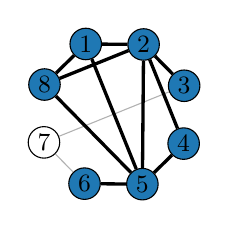
\begin{tikzpicture}[scale=0.8]
        \newcount \c
        \foreach \n in {1, ..., 8}{
            \c=\n \advance\c by -1 \multiply\c by -360 \divide\c by 8 \advance\c by 90 \advance\c by 22.5
            \ifthenelse{\n = 1 \OR \n = 2 \OR \n = 3 \OR \n = 4 \OR \n = 5 \OR \n = 6 \OR \n = 8}{
                \node[selectedvertex] (N\n) at (\the\c:1.2) {\n};
            }{
                \node[plainvertex] (N\n) at (\the\c:1.2) {\n};
            }
        }

        \draw [edge] (N3) -- (N7);
        \draw [edge] (N6) -- (N7);

        \draw [bedge] (N1) -- (N2);
        \draw [bedge] (N1) -- (N5);
        \draw [bedge] (N1) -- (N8);
        \draw [bedge] (N2) -- (N5);
        \draw [bedge] (N2) -- (N8);
        \draw [bedge] (N5) -- (N8);
        \draw [bedge] (N2) -- (N3);
        \draw [bedge] (N2) -- (N4);
        \draw [bedge] (N4) -- (N5);
        \draw [bedge] (N5) -- (N6);
    \end{tikzpicture}

    \caption{On the left, a graph, with its unique maximum clique $\{1, 2, 5, 8\}$ of size 4
        highlighted. On the right, the same graph, with a maximum $2$-clique $\{1, 2, 3, 4, 5, 6, 8\}$
        of size 7 highlighted. This is not a $2$-club, since the only path of length 2 between vertices 3 and 6
        goes through vertex 7. A $3$-clique covers the entire graph.}
    \label{figure:k-cliques}
\end{figure}

A recent survey by \citeauthor{Shahinpour:2013} \shortcite{Shahinpour:2013} discusses algorithms and
results for $k$-clique and $k$-club problems.  We adopt their notation of $\tilde{\omega}_k$ for
the size of a maximum $k$-clique; the use of $\omega$ for the size of a maximum clique is standard.
They note that ``unlike the maximum clique problem, the maximum $s$-clique problem has not been the
subject of extensive research and we are not aware of any computational results for this problem to
date''. This is in contrast to the $k$-club problem, for which a wide range of computational results
are available
\cite{Bourjolly:2000,Bourjolly:2002,Mahdavi:2012,Hartung:2012,Chang:2013,Shahinpour:2013,Wotzlaw:2014,Picker:2015,Carvalho:2016}.

A maximum clique algorithm can easily be adapted to find a maximum $k$-clique in a graph $G$ by
considering the graph $G^k$: this graph has the same vertex set as $G$, and edges between any two
distinct vertices $v_1$ and $v_2$ iff there is a path of length at most $k$ between $v_1$ and $v_2$
in $G$. It is easy to see that maximum cliques in $G^k$ correspond with maximum $k$-cliques in $G$
\cite{Balasundaram:2005}.  However, it is not obvious that this is a viable approach: even if $G$ is
sparse, $G^k$ may not be, and the maximum clique problem on dense graphs can be very challenging
computationally. Here we take a state-of-the-art maximum clique algorithm which is suitable for use
on dense graphs \cite{Prosser:2012}, and investigate whether this approach is feasible in practice.
We modify the algorithm to include a new lazy ``global domination'' inference step---this technique
provides no benefit for typical maximum clique problems, but for maximum $k$-clique graphs it
sometimes gives improvements of several orders of magnitude. We present computational results for
the maximum $k$-clique problem on a range of benchmark and real-world graphs. We finish with a
detailed look at random graphs.

Throughout, our graphs are finite, undirected, and contain no loops. If $G$ is a graph with vertex
set $V$ and edge set $E$, we may write $\vertexset(G)$ to mean $V$. The \emph{neighbourhood} of a
vertex $v$ in a graph $G$, written $\neighbourhood_G(v)$, is the set of vertices adjacent to $v$.
The \emph{degree} of a vertex is the cardinality of its neighbourhood. The density of a graph,
denoted $D$, is the proportion of distinct pairs of vertices which have an edge between them. The
subgraph \emph{induced by} a set of vertices $W$ is the subgraph with vertex set $W$, and all edges
from the original graph that are between pairs of vertices in $W$. If $A$ and $B$ are sets of
vertices, we write $A \setminus B$ for the set of vertices which are in $A$ but not $B$, and we
write $A + v$ and $A - v$ for $A \cup \{v\}$ and $A \setminus \{v\}$ respectively.

\section{Algorithms}

Our approach for finding a maximum $k$-clique is presented as \cref{algorithm:maxKClique}. Our first
step (\mcline{power}) is to replace our input graph $G$ with $G^k$. We may construct this graph
using a bounded breadth-first search: we refer to \citeauthor{Chang:2013} \shortcite{Chang:2013} for
how to implement this quickly in practice.

\begin{algorithm}[t]\DontPrintSemicolon
    
\begin{tikzpicture}[remember picture,overlay]
        \coordinate (cvrej1c) at ($(pic cs:cvrej1) + (0, 0.15)$);
        \coordinate (cvrej2c) at ($(pic cs:cvrej2) + (0, 0.00)$);
        \node [fill=safelightblue, rounded corners, fit=(cvrej1c) (cvrej2c)] { };

        \coordinate (cdom1c) at ($(pic cs:cdom1) + (0, 0.15)$);
        \coordinate (cdom2c) at ($(pic cs:cdom2) + (0, -0.10)$);
        \node [fill=safelightblue, rounded corners, fit=(cdom1c) (cdom2c)] { };

        \coordinate (cvinp1c) at ($(pic cs:cvinp1) + (0, 0.15)$);
        \coordinate (cvinp2c) at ($(pic cs:cvinp2) + (1, 0.00)$);
        \node [fill=safelightblue, rounded corners, fit=(cvinp1c) (cvinp2c)] { };

        \coordinate (cvrejg1c) at ($(pic cs:cvrejg1) + (0, 0.15)$);
        \coordinate (cvrejg2c) at ($(pic cs:cvrejg2) + (0, 0.00)$);
        \node [fill=safelightblue, rounded corners, fit=(cvrejg1c) (cvrejg2c)] { };

    \end{tikzpicture}

    \nl $\FuncSty{maxKClique}$ :: (Graph $G$, Integer $k$) $\rightarrow$ Vertex Set \;
    \nl \Begin{
        \nl $G$ $\gets$ $G^k$ \mclabel{power} \;
        \nl permute $G$ into non-increasing degree order \mclabel{permute} \;
        \nl $\KwSty{global}$ $\Cbest$ $\gets$ $\emptyset$ \mclabel{cbest} \;
        \nl $\expand$($\emptyset$, $\vertexset(G)$) \mclabel{c} \mclabel{p} \;
        \nl $\KwSty{return}$ $\Cbest$ (unpermuted) \;
    }
    \vspace{0.5ex}

    \nl $\expand$ :: (Vertex Set $C$, Vertex Set $P$) \;
    \nl \Begin{
        \nl ($\order$, $\bounds$) $\gets$ $\colourOrder$($P$) \mclabel{colouring} \;
        \nl \tikzmark{cvrej1}$\vrej$ $\gets$ $\kwunset$ \tikzmark{cvrej2} \;
        \nl \For{$i$ $\gets$ $|P|$ $\KwSty{downto}$ 1\mclabel{righttoleft}}{
            \nl \lIf{\textnormal{$|C|$ + $\bounds[i]$ $\le$ $|\Cbest|$}\mclabel{bound}}{$\KwSty{return}$}
            \nl \tikzmark{cdom1}\If{\textnormal{$\vrej$ $\ne$ $\kwunset$}}{
                \nl $P$ $\gets$ $P$ $\setminus$ $\dominated(\vrej)$ \tikzmark{cdom2} \mclabel{dominated} \;
            }
            \nl $v$ $\gets$ $\order[i]$ \mclabel{v} \;
            \nl \tikzmark{cvinp1}\If{$v$ $\in$ $P$\tikzmark{cvinp2}\mclabel{alreadyrejected}}{
                \nl $C'$ $\gets$ $C + v$ \mclabel{vinstart} \;
                \nl \lIf{\textnormal{$|C'| > |\Cbest|$}}{$\Cbest$ $\gets$ $C'$\mclabel{unseat}}
                \nl $P'$ $\gets$ $P$ $\cap$ $\neighbourhood_G(v)$ \mclabel{pprime} \;
                \nl \lIf{$P'$ $\ne$ $\emptyset$}{$\expand$($C'$, $P'$)\mclabel{vinend}\mclabel{recurse}}
                \nl $P$ $\gets$ $P - v$\tikzmark{creject2} \mclabel{vnotin} \;
            }
            \nl \tikzmark{cvrejg1}$\vrej$ $\gets$ $v$ \tikzmark{cvrejg2} \mclabel{vrej} \;
        }
    }
    \vspace{0.5ex}

    \nl $\colourOrder$ :: (Vertex Set $P$) $\rightarrow$ (Vertex Array, Int Array) \;
    \nl \Begin{
        \nl ($\order$, $\bounds$) $\gets$ ($[]$, $[]$) \;
        \nl $\uncoloured$ $\gets$ $P$ \;
        \nl $\colour$ $\gets$ $1$ \mclabel{colour1} \;
        \nl \While{$\uncoloured$ $\ne$ $\emptyset$\mclabel{uncoloured}}{
            \nl $\colourable$ $\gets$ $\uncoloured$ \mclabel{currentcolourstart} \;
            \nl \While{$\colourable$ $\ne$ $\emptyset$}{
                \nl $v$ $\gets$ the first vertex of $\colourable$ \;
                \nl append $v$ to $\order$ \;
                \nl append $\colour$ to $\bounds$ \;
                \nl $\uncoloured$ $\gets$ $\uncoloured - v$ \;
                \nl $\colourable$ $\gets$ $\colourable \setminus \neighbourhood_G(v)$ \mclabel{currentcolourend}\mclabel{notcolourable}\;
            }
            \nl $\colour$ $\gets$ $\colour + 1$ \mclabel{colourplus1}
        }
        \nl $\KwSty{return}$ ($\order$, $\bounds$) \;
    }
    \vspace{0.5ex}

    \nl $\dominated$ :: (Vertex $v$) $\rightarrow$ Vertex Set \;
    \nl \Begin{
        \nl $\KwSty{return}$ $\{ w \in \vertexset(G) : \neighbourhood_G(w) - v \subseteq \neighbourhood_G(v) - w \} $\;
    }
    \caption{Solving the maximum $k$-clique problem.}
    \label{algorithm:maxKClique}
\end{algorithm}

\paragraph{Colouring}

The current state-of-the-art for the maximum clique problem on dense graphs, due to Tomita et al.\
\cite{Tomita:2007,Tomita:2010}, is to use branch and bound with a greedy graph
colouring.  A \emph{colouring} of a graph is an assignment of colours to vertices, such that
adjacent vertices are given different colours; if we can colour a graph using $c$ colours, then the
graph cannot contain a clique of size greater than $c$ (each vertex in a clique must be given a
different colour).

Obtaining a minimal colouring is \NP-hard, but we may create a greedy colouring in polynomial time.
This is done by the $\colourOrder$ routine: we start the first colour (\mcline{colour1}), and while
there are uncoloured vertices remaining (\mcline{uncoloured}), we try to give each vertex in turn
the current colour (\mclinerange{currentcolourstart}{currentcolourend}).  When we cannot colour any
further vertices, we start a new colour (\mcline{colourplus1}).

The key step in \citeauthor{Tomita:2010}'s algorithms is to produce a constructive colouring---the
$\colourOrder$ routine does not just return the number of colours used. Instead, it returns a pair
of arrays, $\order$ and $\bounds$. The $\order$ array contains vertices, in the order in which they
were coloured. The $i$th entry of the $\bounds$ array contains the colour number used for the $i$th
vertex in $\order$. We illustrate this in \cref{figure:colours}. Crucially, $\bounds$ is
non-decreasing (i.e.\ $\bounds[i+1] \ge \bounds[i]$), and we may colour the subgraph induced by the
first $i$ vertices of $\order$ using $\bounds[i]$ colours.

\begin{figure}[b]
    \centering
    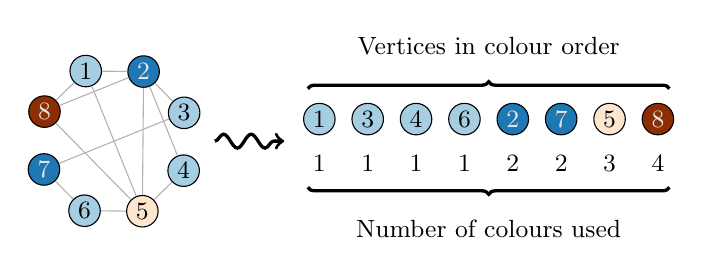
\begin{tikzpicture}[scale=0.8]
\newcount \c
\foreach \n in {1, ..., 8}{
    \c=\n \advance\c by -1 \multiply\c by -360 \divide\c by 8 \advance\c by 90 \advance\c by 22.5
    \ifthenelse{\n = 1 \OR \n = 3 \OR \n = 4 \OR \n = 6}{
        \node[vertexc1] (N\n) at (\the\c:1.2) {\n};
    }{}
    \ifthenelse{\n = 2 \OR \n = 7}{
        \node[vertexc2] (N\n) at (\the\c:1.2) {\n};
    }{}
    \ifthenelse{\n = 5}{
        \node[vertexc3] (N\n) at (\the\c:1.2) {\n};
    }{}
    \ifthenelse{\n = 8}{
        \node[vertexc4] (N\n) at (\the\c:1.2) {\n};
    }{}
}

\draw [edge] (N2) -- (N3);
\draw [edge] (N2) -- (N4);
\draw [edge] (N3) -- (N7);
\draw [edge] (N4) -- (N5);
\draw [edge] (N5) -- (N6);
\draw [edge] (N6) -- (N7);
\draw [edge] (N1) -- (N2);
\draw [edge] (N1) -- (N5);
\draw [edge] (N1) -- (N8);
\draw [edge] (N2) -- (N5);
\draw [edge] (N2) -- (N8);
\draw [edge] (N5) -- (N8);

\draw [processarrow] (1.6, 0) -> (2.7, 0);

\coordinate (Ms) at (3.0, 0.35);
\node[right = 0.0 of Ms, vertexc1] (M1) {1};
\node[right = 0.2 of M1, vertexc1] (M2) {3};
\node[right = 0.2 of M2, vertexc1] (M3) {4};
\node[right = 0.2 of M3, vertexc1] (M4) {6};
\node[right = 0.2 of M4, vertexc2] (M5) {2};
\node[right = 0.2 of M5, vertexc2] (M6) {7};
\node[right = 0.2 of M6, vertexc3] (M7) {5};
\node[right = 0.2 of M7, vertexc4] (M8) {8};

\draw[brace] ($(M1.north west)+(0.0,0.3)$) -- ($(M8.north east)+(0.0,0.3)$);
\node[anchor=south, label] at ($(M1)!0.5!(M8)$)[yshift=0.7cm] { Vertices in colour order };

\coordinate (Bs) at (3.0, -0.35);
\node[right = 0.0 of Bs, notvertex] (B1) {1};
\node[right = 0.2 of B1, notvertex] (B2) {1};
\node[right = 0.2 of B2, notvertex] (B3) {1};
\node[right = 0.2 of B3, notvertex] (B4) {1};
\node[right = 0.2 of B4, notvertex] (B5) {2};
\node[right = 0.2 of B5, notvertex] (B6) {2};
\node[right = 0.2 of B6, notvertex] (B7) {3};
\node[right = 0.2 of B7, notvertex] (B8) {4};

\draw[brace] ($(B8.south east)+(0.0,-0.2)$) -- ($(B1.south west)+(0.0,-0.2)$);
\node[anchor=north, label] at ($(B1)!0.5!(B8)$)[yshift=-0.6cm] { Number of colours used };
    \end{tikzpicture}

    \caption{The graph on the left has been coloured greedily, using four
        colours: vertices 1, 3, 4 then 6 were given the first colour, then
        vertices 2 then 7 were given the second colour, then vertex 5 was given
        the third colour, and vertex 8 the fourth colour. The $\order$ array,
        on top, contains the vertices in the order they were coloured; the
        $i$th entry of the $\bounds$ array, below, contains the number of colours
        used to colour the first $i$ vertices of $\order$.}
    \label{figure:colours}
\end{figure}

The order in which vertices are selected for colouring can have a large effect upon performance.
Various initial vertex orderings have been considered for the maximum clique problem
\cite{Prosser:2012,DBLP:conf/lion/SegundoLB14}. Here we will colour vertices in a static
non-increasing degree order, which we do by permuting the graph at the top of search
(\mcline{permute}). We will \emph{not} be using a dynamic tie-breaking mechanism: although doing so
can sometimes be beneficial for small dense graphs in a maximum clique context \cite{Tomita:2010},
for the larger graphs we will be considering here the cubic cost is prohibitively expensive. For the
same reason, and additionally because our colour classes typically contain many vertices, we use a
simple greedy colouring and do not use a colour repair step \cite{Tomita:2010} or stronger
MaxSAT-based inference \cite{DBLP:journals/cor/SegundoNB15,DBLP:conf/lion/LiJX15}.

\paragraph{Branching and recursing}

We may now describe the main recursive part of the algorithm. If $v$ is a vertex, then a clique in
$G^k$ either contains only $v$ and vertices adjacent to $v$, or does not contain $v$. This allows us
to grow cliques by repeatedly picking a vertex, and branching upon whether or not to include it. Our
growing clique is stored in the variable $C$, which is initially empty (\mcline{c}). We also track
which vertices may still be added to $C$ in the variable $P$, which initially contains every vertex
(\mcline{p}). The $\expand$ procedure picks a vertex $v$ (\mcline{v}), then considers adding $v$ to
$C$ (\mclinerange{vinstart}{vinend}): we create a new $P'$ from $P$ (\mcline{pprime}) by
rejecting vertices which are not adjacent to $v$ (and thus every vertex in $P'$ is adjacent to
\emph{every} vertex in $C$). If vertices remain in $P'$, we recurse (\mcline{recurse}). We then take
the opposite branch choice, and consider rejecting from $P$ and $C$
(\mcline{vnotin}). We then loop, and pick a new $v$.

\paragraph{Integrating the colour bound}

We keep track of the best solution we have found so far, which we call the \emph{incumbent}; this is
stored in $\Cbest$, which is initially empty (\mcline{cbest}). Whenever we find a new clique, we
compare its size to that of $\Cbest$, and if it is better, the incumbent is unseated
(\mcline{unseat}). Now we may make use of the colour bound. At the start of the recursive procedure
(\mcline{colouring}), we use $\colourOrder$ to produce a constructive greedy colouring of the
subgraph induced by $P$ into the array $\order$, with the colour numbers placed in $\bounds$. When
selecting $v$, we iterate over $\bounds$ from right to left (\mcline{righttoleft}). Now on
\mcline{bound} we know that the largest possible clique we could find at the current location has
size no greater than $|C| + \bounds[i]$, so if this cannot unseat the incumbent then we may abandon
search and backtrack.

\paragraph{Lazy global domination}

Aside from the $G^k$ step, what we have described so far is a standard maximum clique algorithm, and
all we have done is opted out of certain more computationally expensive inference steps (more
complicated initial vertex orderings, and cubic colourings). If we ignore the lines shown in blue,
we obtain the maximum clique algorithm variation that \citeauthor{Prosser:2012}
\shortcite{Prosser:2012} calls ``MCSa1''.  Now we will introduce a new lazy global domination rule
which performs additional inference during search. This rule is not specific to the maximum
$k$-clique problem, and is also valid for the maximum clique problem.

Let $v$ and $w$ be distinct vertices in a graph $G$. We say that $v$ \emph{dominates} $w$ if the
neighbourhood of $w$, excluding $v$, is a (possibly non-strict) subset of the neighbourhood of $v$,
excluding $w$. From a maximum clique perspective, this means that $v$ is ``better than'' $w$. If $v$
and $w$ are adjacent, any clique containing $w$ may always be extended by the inclusion of $v$; if
$v$ and $w$ are non-adjacent, replacing $w$ with $v$ in any clique containing $w$ cannot reduce the
amount by which the clique may be grown.

Suppose a graph does contain one or more pairs of dominating vertices. We could make use of this
fact during search in at least two ways. Firstly, when accepting a vertex $w$, we may also
unconditionally accept any vertex $v$ which both dominates and is adjacent to $w$. Secondly, when
rejecting a vertex $v$, we may also unconditionally reject any vertex $w$ which is dominated by $v$.
We could also choose to calculate domination globally (i.e.\ with respect to $G^k$, or even the
original $G$), or locally (i.e.\ with respect to the subgraph of $G^k$ induced by $C \cup P$).

Detecting whether one vertex dominates another may be done in linear time (we discuss this further
below), but finding all vertices dominated by a particular vertex is quadratic, and finding all
dominations is cubic. This is a heavy price to pay, if there are no dominating vertices.  This is
why such a rule has not previously been used in the maximum clique context: in the authors'
experience, most graphs typically considered for the maximum clique problem do not contain
dominating vertices, and those that do are too easy computationally for the step to be worthwhile.

However, some of the graphs we consider in the following section \emph{do} contain dominating
vertices, and although the maximum clique problem is trivial on these graphs, the maximum $k$-clique
problem is not for some values of $k$. Preliminary experiments suggested that the use of a
domination rule could be extremely beneficial in certain circumstances, but that in cases where it
had little effect, doing such a calculation introduced a substantial penalty to runtimes. Moreover,
even in graphs where dominating vertices are present, knowing this fact is sometimes not useful: it
is common for an optimal solution to be found straight away, and for the bound to be strong enough
to prove optimality immediately, so no branching occurs.

This motivates the design of a lazy global domination rule. We perform our domination checks
globally, with respect to $G^k$ (which may contain more dominating vertices than $G$), and we
remember and reuse the results of any domination checks we perform. We also only perform inference
on the ``reject'' case, to avoid introducing any cost when a solution is found and proven optimal
without branching.

The lines marked in blue in \cref{algorithm:maxKClique} show how this is done. When a vertex $\vrej$
is rejected, we remove from $P$ any vertex that is dominated (with respect to $G^k$) by $\vrej$.
This is \mcline{dominated}; the set of dominated vertices calculated here should be cached.  One
might expect that this calculation would appear after \mcline{vnotin}. However, this introduces a
cost if the bound allows the next choice of $v$ to be eliminated. Thus we simply remember that we
have rejected $v$ by storing it in $\vrej$ (\mcline{vrej}), and lazily postpone the filtering until
after the bound has been checked.

Finally, note that we do not perform a new colouring when we reject dominated vertices---doing so
typically does not lead to a smaller bound, since most colour classes contain many vertices. Thus
when we select a $v$ from $\order$, it is now possible that $v$ has already been rejected. We check
for this on line \mcline{alreadyrejected}.

\paragraph{Bitset encoding} San Segundo et al.\ \shortcite{SanSegundo:2011,SanSegundo:2013} observed
that the performance of Tomita's algorithms could be enhanced substantially by using a bitset
encoding to obtain a form of SIMD-like parallelism, without altering the steps taken. We have taken
such an approach here too, although we do not describe it explicitly---when permuting $G$ on line
\mcline{permute}, the graph should be re-encoded as an array of adjacency bitsets. (It is not
helpful to do this before constructing $G^k$.) Now the intersection on \mcline{pprime} becomes a
simple bitwise ``and'' operation, and the intersection with complement on \mcline{notcolourable} is
a bitwise ``and not'' operation. This is beneficial when testing for dominance, too: each bit in the
dominated set on \mcline{dominated} may be determined by a bitwise ``and not'', unsetting a bit, and
testing whether the result is empty; the set difference is again a bitwise ``and not'' operation.

\section{Experimental Results}

We now give experimental results on a range of standard benchmarks, and on real-world and random
graphs. Experiments were run on a machine with dual 3.1GHz Intel E5-2687W v3 processors and
256GBytes RAM; single-threaded runtimes are given, except in \cref{table:parallel}, where 20 threads
were used (our machine does not have hyper-threading enabled). Our software was implemented in C++,
using C++11 native threads, and was compiled using GCC 5.1.0. The time taken to read in the graph
from a file is excluded, but preprocessing time (including the construction of $G^k$ and the bitset
encoding) is included. We use the term \emph{nodes} to refer to the number of recursive calls made
by the branch-and-bound part of the algorithm.

\subsection{Real-World Graphs}

We begin with a selection of real-world and standard benchmark graphs. We look at $k$ equal to 2, 3
and 4 in every case---this is a standard practice for the $k$-club problem.

\paragraph{Erd\H{o}s collaboration graphs}

In \cref{table:erdos} we present experimental results from Erd\H{o}s
collaboration graphs from the Pajek dataset by Vladimir Batagelj and Andrej
Mrvar\footnote{http://vlado.fmf.uni-lj.si/pub/networks/data/}.  We were able to solve all of
these problems in under four minutes (and all but three in under four seconds) when using the
domination rule. However, using the unmodified maximum clique algorithm, three of these results did
not finish running within one hour. Note that for $k = 4$, a $k$-clique covers all of ``Erdos02''.

\begin{table}
    \scriptsize\setlength{\tabcolsep}{5pt} % carefully tuned!
    \centering
    \begin{tabular}{l c rr rr rr}
        \toprule
        & & & & \multicolumn{2}{c}{Unmodified} & \multicolumn{2}{c}{With Domination} \\
    \cmidrule(lr){5-6}
    \cmidrule(lr){7-8}
    Instance & \multicolumn{1}{c}{$k$} & \multicolumn{1}{c}{$D$} & \multicolumn{1}{c}{$\tilde{\omega}_k$} &
    \multicolumn{1}{c}{Nodes} & \multicolumn{1}{c}{Time} &
    \multicolumn{1}{c}{Nodes} & \multicolumn{1}{c}{Time} \\
    \midrule
    \inputhaxx{gen-table-erdos}
    \bottomrule
\end{tabular}
\caption{Experimental results for Erd\H{o}s collaboration graphs. For each
graph, we consider $k$ equal to 2, 3 and 4. In each case we show the density of
$G^k$, the size of a maximum $k$-clique, and then for both the unmodified
algorithm and the algorithm with our lazy global domination step, the number of
nodes required, and the runtime in seconds.}\label{table:erdos}
\end{table}

In several cases, the algorithm found and proved an optimal solution immediately ($\tilde{\omega}_k$
is equal to the number of search nodes). This illustrates the necessity of laziness: if we simply
computed dominating pairs upfront, we would be paying a cubic preprocessing cost for an algorithm
which is effectively quadratic in practice.

By comparing these results with the $k$-club results of Chang et al.\ \shortcite{Chang:2013}, we see
that in all but four cases the $k$-clique and $k$-club numbers are equal; all of these differences
occur when $k = 4$. (Chang et al.\ did not investigate the ``Erdos02'' graph, but
\citeauthor{Wotzlaw:2014} confirmed privately that the $k$-clique and $k$-club numbers are the same
here too.) On the other hand, the $k$-clique numbers are sometimes much easier to find, both
algorithmically and computationally.

\paragraph{Clique graphs}

In \cref{table:clique} we present results from the ``clique'' graphs from the
Second DIMACS implementation challenge\footnote{http://dimacs.rutgers.edu/Challenges/}. These
graphs were designed to test maximum clique implementations. Nearly all of these graphs have
diameter 2, so a 2-clique covers the entire graph---we have ignored these. The only exceptions are
the ``c-fat'' family (all of which are trivial for a maximum clique solver), and one of the
``p\_hat'' graphs.

\begin{table}
    \scriptsize\setlength{\tabcolsep}{5pt} % carefully tuned!
    \centering
    \begin{tabular}{l c rr rr rr}
        \toprule
        & & & & \multicolumn{2}{c}{Unmodified} & \multicolumn{2}{c}{With Domination} \\
    \cmidrule(lr){5-6}
    \cmidrule(lr){7-8}
    Instance & \multicolumn{1}{c}{$k$} & \multicolumn{1}{c}{$D$} & \multicolumn{1}{c}{$\tilde{\omega}_k$} &
    \multicolumn{1}{c}{Nodes} & \multicolumn{1}{c}{Time} &
    \multicolumn{1}{c}{Nodes} & \multicolumn{1}{c}{Time} \\
    \midrule
    \inputhaxx{gen-table-dimacs}
    \bottomrule
\end{tabular}
\caption{Experimental results for DIMACS clique graphs with diameter greater
    than two.}\label{table:clique}
\end{table}

With the domination rule, we solve all of these problems within a tenth of a second. Without, two of
the results take over an hour, and the rest remain trivial. Note that in several cases, for some
values of $k$ a $k$-clique covers the entire graph.  Again using Chang et al.'s results, we see that for the first six graphs in this table the $k$-clique and $k$-club
numbers are the same for each value of $k$ (Chang et al.\ did not investigate ``c-fat500-10'' or
``p-hat300-1'').

\paragraph{Partitioning graphs}

\Cref{table:partitioning} presents results from the smallest 20 partitioning graphs
from the 10th DIMACS Implementation
Challenge\footnote{http://staffweb.cms.gre.ac.uk/\textasciitilde{}wc06/partition/}.  Many of these graphs are
considerably larger than those typically considered for the maximum clique problem, and we might
expect our $O(|V|^2)$ memory requirements to cause problems. Nonetheless, with the domination rule
there is only one instance which we were unable to solve within an hour (and without the domination
rule, there are two).

\begin{table}
    \scriptsize\setlength{\tabcolsep}{3.5pt} % carefully tuned!
    \setlength{\aboverulesep}{-0.4pt} % this only affects the cmidrules on this table
    \centering
    \begin{tabular}{l c rr rr rr}
        \toprule
        & & & & \multicolumn{2}{c}{Unmodified} & \multicolumn{2}{c}{With Domination} \\
        \cmidrule(lr){5-6} \cmidrule(lr){7-8}
    Instance & \multicolumn{1}{c}{$k$} & \multicolumn{1}{c}{$D$} & \multicolumn{1}{c}{$\tilde{\omega}_k$} &
    \multicolumn{1}{c}{Nodes} & \multicolumn{1}{c}{Time} &
    \multicolumn{1}{c}{Nodes} & \multicolumn{1}{c}{Time} \\
    \midrule
    \inputhaxx{gen-table-dimacs10walshaw}
    \bottomrule
\end{tabular}
    \caption{Results for smaller DIMACS partitioning graphs.}\label{table:partitioning}
\end{table}

On the other hand, we sometimes see a significant cost where the domination rule does not help, and
where the proof of optimality is not immediate: in ``3elt'' and ``4elt'', our runtimes can nearly
double, and for ``cs4'' and ``cti'' the slowdown is sometimes over a factor of ten. Thus laziness
can be costly when the rule is used, but useless.

Five of these graphs were considered for the $k$-club problem by Wotzlaw \shortcite{Wotzlaw:2014}.
In every case, the $k$-clique and $k$-club numbers are the same. However, the $k$-clique number was
again consistently much easier to find.

\paragraph{Clustering graphs}

\Cref{table:clustering} presents results from the smallest 20 clustering graphs
from the 10th DIMACS Implementation
Challenge\footnote{http://www.cc.gatech.edu/dimacs10/archive/clustering.shtml}. Again, from a
maximum clique perspective these would be considered unusually large graphs. However, only five were
unsolvable within an hour (plus a further two when the domination rule was not used), and over half of the
problems took under two seconds.

\begin{table}
    \scriptsize\setlength{\tabcolsep}{3.8pt} % carefully tuned!
    \setlength{\aboverulesep}{-0.4pt} % this only affects the cmidrules on this table
    \centering
    \begin{tabular}{l c rr rr rr}
        \toprule
        & & & & \multicolumn{2}{c}{Unmodified} & \multicolumn{2}{c}{With Domination} \\
    \cmidrule(lr){5-6}
    \cmidrule(lr){7-8}
    Instance & \multicolumn{1}{c}{$k$} & \multicolumn{1}{c}{$D$} & \multicolumn{1}{c}{$\tilde{\omega}_k$} &
    \multicolumn{1}{c}{Nodes} & \multicolumn{1}{c}{Time} &
    \multicolumn{1}{c}{Nodes} & \multicolumn{1}{c}{Time} \\
    \midrule
    \inputhaxx{gen-table-dimacs10cluster}
    \bottomrule
\end{tabular}
\caption{Results for smaller DIMACS clustering graphs.}\label{table:clustering}
\end{table}

Seven of these graphs were considered for the $k$-club problem by Wotzlaw \shortcite{Wotzlaw:2014}.
In these cases, the $2$-clique and $2$-club numbers are the same, except for ``football'' where the
$2$-club number is 16 but the $2$-clique number is 17; for $k = 3$ and $k = 4$ there are some
differences. There is a large difference in computational difficulty between the $k$-clique and
$k$-club problems: for ``polblogs'' with $k = 3$ and $k = 4$, Wotzlaw was unable to prove optimality
within an hour, but we required less than two seconds to do so. In both of these cases the
$k$-clique and $k$-club numbers are the same.

\subsection{Parallel Search}

\begin{table}
    \scriptsize\setlength{\tabcolsep}{3.4pt} % carefully tuned!
    \centering
    \begin{tabular}{l c rr rr rr}
        \toprule
        & & & & \multicolumn{2}{c}{Sequential} & \multicolumn{2}{c}{Parallel} \\
    \cmidrule(lr){5-6}
    \cmidrule(lr){7-8}
    Instance & \multicolumn{1}{c}{$k$} & \multicolumn{1}{c}{$D$} & \multicolumn{1}{c}{$\tilde{\omega}_k$} &
    \multicolumn{1}{c}{Nodes} & \multicolumn{1}{c}{Time} &
    \multicolumn{1}{c}{Nodes} & \multicolumn{1}{c}{Time} \\
    \midrule
    \inputhaxx{gen-table-parallel}
    \bottomrule
\end{tabular}
\caption{Experimental results for multi-threaded search on harder instances, using 20 threads. For
    each graph, we consider $k$ equal to 2, 3 and 4. In each case we show the
    density of $G^k$, the size of a maximum $k$-clique, and then for both the
    sequential algorithm and the parallel algorithm (with lazy global domination in both cases),
    the number of nodes required, and the runtime in seconds.}\label{table:parallel}
\end{table}

Parallel search is an active research area for maximum clique algorithms
\cite{DBLP:journals/algorithms/McCreeshP13,DBLP:journals/jcisd/DepolliKRTJ13,DBLP:journals/topc/McCreeshP15,DBLP:journals/cor/SegundoLP16}.
The idea is to work with a shared incumbent, and to speculatively explore portions of the search
tree in parallel using multiple threads, in the hopes that most of the speculative work will
contribute to the optimality proof.

We selected the four graphs which we were unable to solve (for some values of $k$), along with two
of the challenging graphs which required substantial amounts of search (at least half a million
nodes) to solve, and repeated the experiments using parallel search with 20 threads and the
domination rule (with the laziness made thread-safe) enabled, using the resplitting strategy
described by \citeauthor{DBLP:journals/topc/McCreeshP15} \shortcite{DBLP:journals/topc/McCreeshP15}.
The results are shown in \cref{table:parallel}. Parallel search allowed us to close two more
instances, and gave improved bounds on the four remaining instances within 12 hours. However, to
get sufficient work balance, we had to allow for work splitting to depth 10 rather than depth 3. A
close inspection of the search patterns showed that simpler static decomposition approaches
\cite{DBLP:journals/jcisd/DepolliKRTJ13,DBLP:journals/cor/SegundoLP16} would give little to no
speedup on many harder $k$-clique instances, unless it were somehow possible to generate
$\mathcal{O}(|V|^{10})$ subproblems.

For the easier instances where the sequential runtime is known, the parallel search did more
work---this is to be expected, since the work distribution approach we used recomputed parts of the
search space (to allow for more efficient mutable data structures to be used during search), and
speculative parallelism is unlikely to contribute to the solution when the sequential search tree is
small. However, despite the extra work, and despite having to introduce overhead into early stages
of the algorithm to allow for work stealing, and despite having more processing power but not more
memory bandwidth, in no cases were the parallel runtimes substantially longer than the sequential
runtimes (although in many cases they were not substantially better either). We also did not
parallelise the construction of $G^k$ or the preprocessing stage of the algorithm, which in many
cases dominated the runtime.

As well as improving the results on the instances we could not solve sequentially, parallel search
sometimes gave large improvements for the easier instances. For ``wing-nodal'' with $k=4$, the
parallel run did much less work than the sequential run: a speedup of over 100 was obtained from 20
cores. A similar effect occurred with ``cond-mat'' and $k=4$. This is because the work splitting
mechanism we used explicitly diversifies at the top of search first, where branching heuristics are
least likely to be correct, which leads to an initial incumbent being found faster---this is in line
with recent observations that tailored work stealing should be favoured over randomised work
stealing for combinatorial search problems
\cite{DBLP:conf/cp/ChuSS09,DBLP:journals/topc/McCreeshP15}.

\subsection{Random Graphs}

\begin{figure}[t]
    \centering
    \input{gen-graph-omega}
    \caption{Values of $\tilde{\omega}_k$ for random graphs $G(200, p)$, with varying edge probabilities.
        We see that even for very low edge probabilities, a maximum $k$-clique
    quickly covers the entire graph when $k > 1$.}
    \label{figure:graph-omega}
\end{figure}

\begin{figure}[t]
    \centering
    \input{gen-graph-nodes}
    \caption{Search space size for random graphs $G(200, p)^k$, with varying edge probabilities. We see that
        $4$-clique is easier than $3$-clique in practice, which in turn is easier than $2$-clique. (The
        complexity peak for maximum clique occurs at around edge probability 0.9, and requires
        approximately 15 million search nodes.)}
    \label{figure:graph-nodes}
\end{figure}

An Erd\H{o}s-R\'{e}nyi random graph $G(n, p)$ has $n$ vertices, and an edge between each distinct
pair of vertices with probability $p$, chosen independently. We now investigate the size of a
maximum $k$-clique in such graphs, and the complexity of finding it. In each case, we use an average
over 100 samples for every point.  We do not use the domination rule for these experiments: the
probability of random graphs having dominating vertices is very low.

In \cref{figure:graph-omega} we illustrate the average value of $\tilde{\omega}_k$ in $G(200,
p)$ for different values of $k$, and a range of values of $p$ for the $x$-axis. We see that even for
very low edge probabilities, a maximum $k$-clique quickly covers the entire graph.  (This is in contrast to
the maximum clique problem, where a maximum clique does not even cover a quarter of the graph for
edge probabilities below 0.75.) In \cref{figure:graph-nodes} we show the average size of the
search space (number of nodes, or recursive calls made) for the same problem. We see that there is a
complexity peak for each $k$, although the peak is much smaller for $k = 4$ than it is for $k = 3$,
which is in turn much smaller than it is for $k = 2$. The peak also occurs for lower edge
probabilities as $k$ increases. For contrast, for the maximum clique problem, the peak occurs at
around edge probability 0.9, and is two orders of magnitude larger.

In \cref{figure:graph-omega-2,figure:graph-nodes-2} we show the effect of
changing $n$ and fixing $k = 2$. As $n$ increases from 50 to 200, the complexity peak becomes much
more pronounced, and shifts slightly towards the left (lower edge probabilities).

\begin{figure}[t]
    \centering
    \input{gen-graph-omega-2}
    \caption{The size of a maximum $2$-clique in random graphs $G(n, p)$ with varying edge
        probabilities, and different values of $n$. For $G(50, p)$, a $2$-clique has size average 50
    from $p = 0.42$ onwards.}
    \label{figure:graph-omega-2}
\end{figure}

\begin{figure}[t]
    \centering
    \input{gen-graph-nodes-2}
    \caption{The search space size for the maximum $2$-clique problem in random graphs $G(n, p)$
        with varying edge probabilities, and for different values of $n$. As $n$ increases, the
    complexity peak grows and moves slowly to the left.}
    \label{figure:graph-nodes-2}
\end{figure}

\section{Conclusion}

We have shown that using a maximum clique algorithm to solve the maximum $k$-clique algorithm for a
graph $G$ by considering $G^k$ in place of $G$ is feasible in practice. This is despite $G^k$
potentially being dense even if $G$ is sparse---this ruled out the use of maximum clique algorithms
which are designed for sparse graphs
\cite{DBLP:conf/waw/PattabiramanPGLC13,DBLP:journals/cor/SegundoLP16}, and we were working with
graphs with many more vertices than is typical for dense maximum clique algorithms.

We introduced a new lazy global domination rule. This was sometimes extremely beneficial, leading to
exponential reductions in the search space---without this rule, we would have been unable to solve
nine of the problem instances we considered, and many others would have taken much longer. However,
even with laziness there is still sometimes a cost to pay when this rule does nothing. This rule is
thus harmful (although only by a polynomial factor) for the graphs typically considered for the
maximum clique problem, and we see the benefit of tailoring algorithms to the problem being solved.
We suggest that a similar rule may also be useful for the maximum $k$-club problem.

We were able to use parallelism to close two further instances, although this required a much finer
level of task granularity than usual.  We suspect further progress could be made by tailoring the
initial vertex ordering based upon what we know about the graphs, or by increasing the number of
recursive calls per second by making the colouring stage cheaper, for example by reusing colour
classes \cite{DBLP:conf/lion/NikolaevBS15}.

Quite often, we saw $k$-clique numbers and $k$-club numbers being the same. However, solving the
maximum $k$-clique problem is much easier, both in terms of the algorithm and computationally. Thus
it is worth checking whether the simpler model would be sufficient for practical applications before
trying to solve the $k$-club problem.

In random graphs, we saw that $G(n, p)^k$ is easier than $G(n, p')$ with some higher probability
$p'$. We also saw that as $k$ increases, the problem gets easier---this was not typically the case
for some of the real world graphs.

Our results suggest that $k$ is a very coarse grained parameter. We saw that often a $2$-clique or
$3$-clique would cover the entire graph. In these circumstances the increased restrictions for
$k$-club are of no benefit. It is not obvious if somehow allowing a ``fractional'' value of $k$
could give more fine-grained control. Thus it may be worth considering other clique relaxations not
based upon distance (although other models also have problems: a density-based relaxation known as
quasi-clique, for example, can allow vertices with only a single edge to be added to a ``clique''
\cite{Abello:2002}).

\bibliographystyle{aaai}
\bibliography{paper}

\end{document}
